\documentclass[a4paper, 12pt]{article}
\usepackage{listings} 
\usepackage{xcolor}
\usepackage{mdframed}
\usepackage{graphicx}
\usepackage{pgfplots}
\usepackage{float}
\usepackage{mathtools}

% Specific Line Breaks
% See https://tex.stackexchange.com/questions/26174/ for details
\usepackage[british]{babel} 

% Page Margins
\usepackage[margin=1.00in]{geometry}

% Large, array-sized, ceiling and floor operators
\DeclarePairedDelimiter\ceil{\lceil}{\rceil}
\DeclarePairedDelimiter\floor{\lfloor}{\rfloor}
\definecolor{code-gray}{gray}{0.93}

% Beginning of Document
\begin{document}
% Title
\title{ECE 443 - Homework \#6}
\author{Collin Heist}
\date{\today}
\maketitle

\pagenumbering{arabic}

% Beginning of Report
\section{Observations}
\label{sec:observations}

\subsection{GET Method}
\label{sec:get-method}
Wireshark shows the TCP packet sent with a new light setting. You can see in the \textbf{Full request URI} part of the HTTP message that the name and value pair are appended to the address. In this case, it is \textbf{lights=on}.

\begin{figure}[H]
\centering
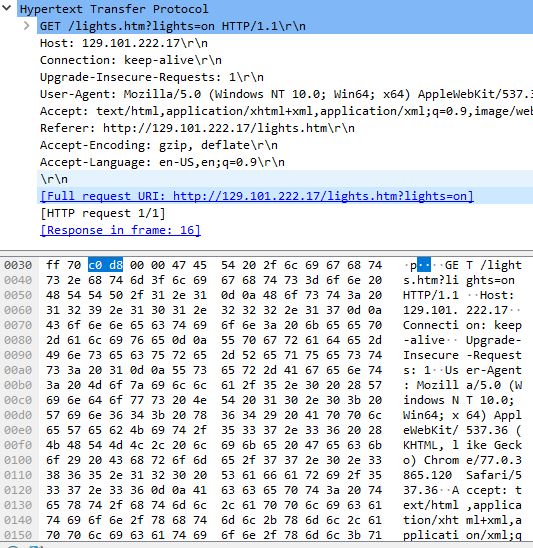
\includegraphics[width=0.8\textwidth]{img-get-wireshark.PNG}
\caption{Wireshark screenshot of the HTTP portion of the TCP packet.}
\label{fig:img-get-wireshark}
\end{figure}

Inside the \textbf{HTTPExecuteGet()} function, the pointer \textbf{ptr} parses this TCP packet to get \emph{just} the value of the light setting, and so the pointer specifically points to the first character in the string ``on''.

\begin{figure}[H]
\centering
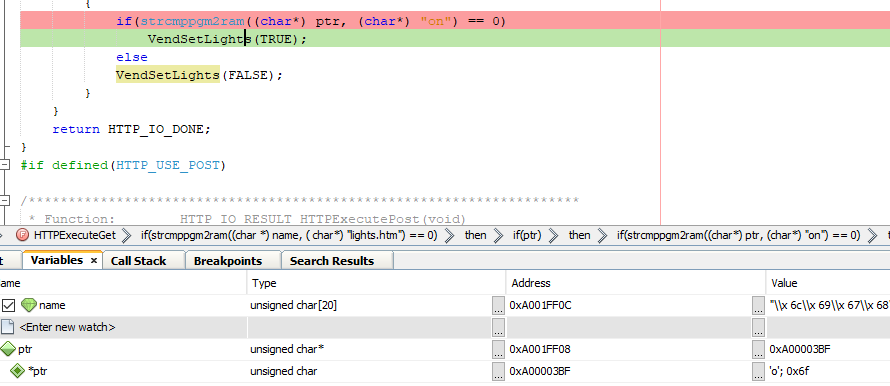
\includegraphics[width=\textwidth]{img-get-variable.PNG}
\caption{MPLab Variable Window showing the value of the pointer for the name / value pair.}
\label{fig:img-get-variable}
\end{figure}

This pointer itself is stored at \textbf{0xA001FF08}, while it points to the memory addres \textbf{0xA00003BF}. Looking at that memory location in the MPLAB Memory View shows the rest of that string. It also shows (in space) the ignored name of the TCP pair (lights). This is in \textbf{Figure~\ref{fig:img-get-memory}}.

\begin{figure}[H]
\centering
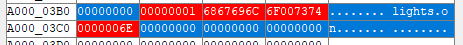
\includegraphics[width=\textwidth]{img-get-memory.PNG}
\caption{MPLab Memory View of the location to which \textbf{ptr} points to -- the value of the name sent through the TCP packet.}
\label{fig:img-get-memory}
\end{figure}

\subsection{POST Method}
\label{sec:post-method}
The POST method sends a lot more data in its TCP packet. Part of this data is shown below, however given there is no real limit to the data-length, not all of it is shown.

\begin{figure}[H]
\centering
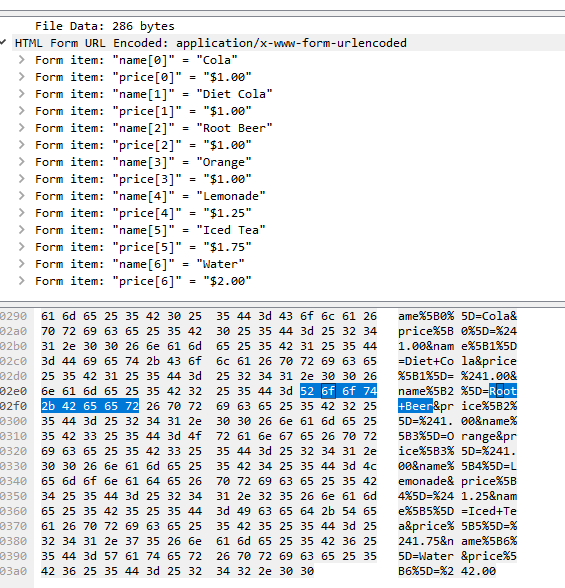
\includegraphics[width=\textwidth]{img-post-wireshark.PNG}
\caption{Wireshark screenshot of the non-encoded HTML form -- contains info on each item on the Product page.}
\label{fig:img-post-wireshark}
\end{figure}

In this case, the name array points to the name of the HTML page making the TCP request. Since the POST method is only used on the \textbf{products.htm} page, we expect the first element in this array to be `p'.

\begin{figure}[H]
\centering
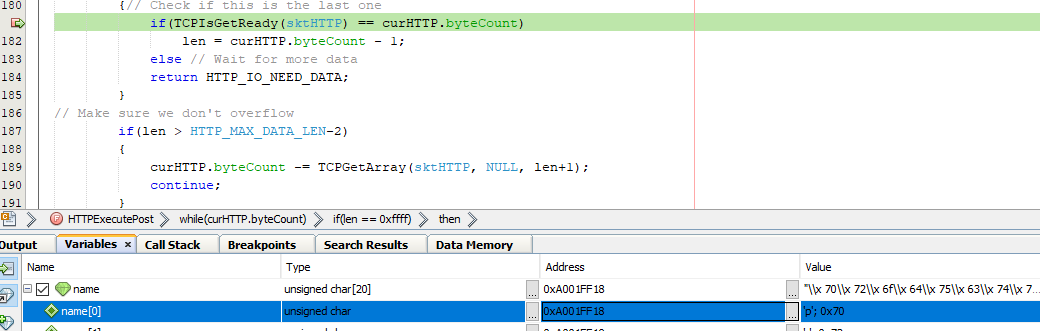
\includegraphics[width=\textwidth]{img-post-variable.PNG}
\caption{MLab Variable Window showing the contents of the \textbf{name} character array that corresponds to which website made the request.}
\label{fig:img-post-varaible}
\end{figure}

And finally, if I look in memory at that array, the full name of the requesting webpage is found to be \textbf{products.htm}. Which is exactly what we expected.

\begin{figure}[H]
\centering
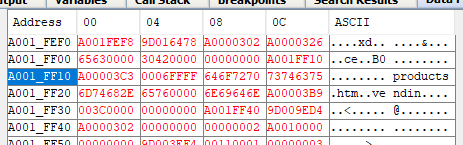
\includegraphics[width=0.8\textwidth]{img-post-memory.PNG}
\caption{MPLab Memory View of the website name array.}
\label{fig:img-post-memory}
\end{figure}

\section{Findings}
Overall, I found the Wireshark program to be really helpful. Being able to capture all the traffic going to a specific IP address made looking at the messages really simple. I think it would have been more useful for me to look close at the structure of the TCP packet -- especially with regard to the POST method. However, for a simple homework like this, it was useful to just easily look at all the information being sent. If there were multiple webpages being served by the PIC, or perhaps many users at a given time, I could see Wireshark being invaluable.

On the other hand, I did not find the memory view particularly helpful, as it seemed to just add a layer of obfuscation on top of the variable window, which was already really helpful. Related to that, it was nice to see the functionality behind the implementation of those GET and POST servicing functions.

\end{document}